\tikzsetnextfilename{hole_ice_models_scatter}%
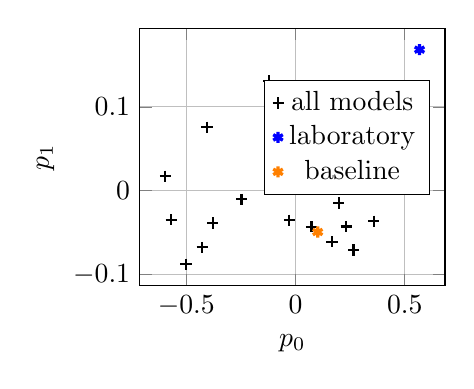
\begin{tikzpicture}
\begin{axis}[
        width=0.45\linewidth, height=0.4\linewidth,
		xmajorgrids, ymajorgrids,
		xlabel=$p_0$,
		ylabel=$p_1$,
		legend columns=1,
		legend style={
			/tikz/every even column/.append style={column sep=0.2cm},
			at={(0.95, 0.8)},
			anchor=north east
		}
        % ytick={-0.1, -0.05, 0, 0.05, 0.1},
        % yticklabels={-0.1, -0.05, 0, 0.05, 0.1}
	]
    \addplot[black, only marks, mark=+, thick] table [x=p0, y=p1] {
       	name	p0	p1
        %nominal	0.567771	0.168269
        h1-100cm	-0.123027	0.131104
        h2-50cm	-0.405128	0.075841
        h3-30cm	-0.595997	0.017468
        dima	0.232258	-0.042754
        dima+	0.265798	-0.070837
        dima-	0.198792	-0.014733
        dragon	0.072961	-0.043175
        greco	0.167150	-0.060809
        %baseline	0.101569	-0.049344
        msu2	0.357705	-0.036428
        martin-0.6-14	-0.028113	-0.035254
        martin-0.8-40	-0.246929	-0.010401
        martin-1.8-125	-0.569511	-0.034839
        all	-0.427318	-0.067581
        tilted	-0.501349	-0.087664
        horizontal	-0.378935	-0.038564
    };
    \addlegendentry{all models}
    \addplot[blue, only marks, mark=asterisk, very thick] coordinates {
        (0.567771,	0.168269)
    };
    \addlegendentry{laboratory}
    \addplot[orange, only marks, mark=asterisk, very thick] coordinates {
        (0.101569,	-0.049344)
    };
    \addlegendentry{baseline}
    

	
\end{axis}
\end{tikzpicture}